\chapter[Deseño]{
  \label{chp:disenho}
  Deseño
}
\minitoc
\newpage

\section{Arquitectura}

A elección de Django coma framework de desenvolvemento obriga a seguir o patrón \textbf{Modelo-Vista-Template}. Este patrón é unha pequena variación do máis coñecido Modelo-Vista-Controlador, que define 3 capas interconectadas co fin de separar a lóxica da aplicación(Vista) do almacenamento dos datos(Modelo) e estas dúas, á súa vez, da interface de usuario(Controlador). A vantaxe que ofrecen os templates de Django é a posibilidade de utilizar os tipos propios do framework para implementar certa lóxica presentacional no renderizado do template.

Neste proxecto, os modelos  definíronse no módulo models.py e as vistas en views.py. Trataranse coma paquetes nos seguintes diagramas. A capa template ven definida no paquete de \say{templates}.

\begin{figure}[h]
	\centering
	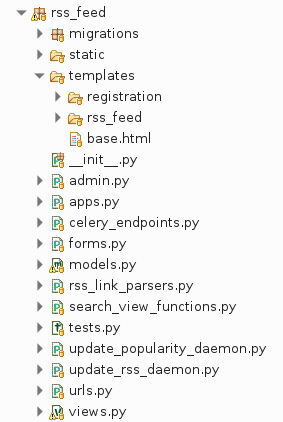
\includegraphics[scale=0.6,keepaspectratio=true]{./images/project_tree.png}
	\caption{Árbore de módulos da aplicación  web.}
	\label{fig:project_tree}
\end{figure}


\subsection{Capa Modelo}

Á hora de definir esta cuestión, tratáronse de respectar as regras do modelo relacional de bases de datos, porén, fixeronse algunhas excepcións motivadas por esixencia da elección do framework Django:

\begin{itemize}
	\item \textbf{Claves primarias subrogadas:} Django encárgase da identificación das tuplas engadindo ás táboas un campo numérico enteiro de incremento automático. Isto utilizarase en todas as táboas sen excepción.
	
	\item \textbf{Relación 1-1:} Como se ve no diagrama Entidade-Relación da figura \ref{fig:diagrama_er}, existe unha relación 1-1 entre a entidade User e a súa entidade feble UserProfile. O motivo da existencia desta última é que se decidiu utilizar a entidade de usuario nativa de Django, co cal fíxose necesaria unha nova táboa para cubrir os atributos de usuario necesarios especificamente para o proxecto. 
\end{itemize}

No \textbf{diagrama Entidade-Relación} da figura \ref{fig:diagrama_er} pódense ver as táboas empregadas sen incluír aquelas automaticamente xeradas para o correcto funcionamento de Django e Celery a excepción da xa mencionada User. Por motivos de claridade, non se incluíron os atributos agás aqueles adicionais nas táboas correspondentes ás relacións N-N.

A estrutura da BD tradúcese na aplicación ás clases definidas no paquete \textbf{models.py} que se ve na figura \ref{fig:clase_models}. Por claridade, nese diagrama de clases só se incluíron os atributos máis representativos ou explicativos das relacións entre clases.

\textbf{Nota:} As entidades e os seus atributos amósanse en detalle no dicionario de datos do anexo \ref{chp:dicionario}.

\begin{figure}[h]
	\centering
	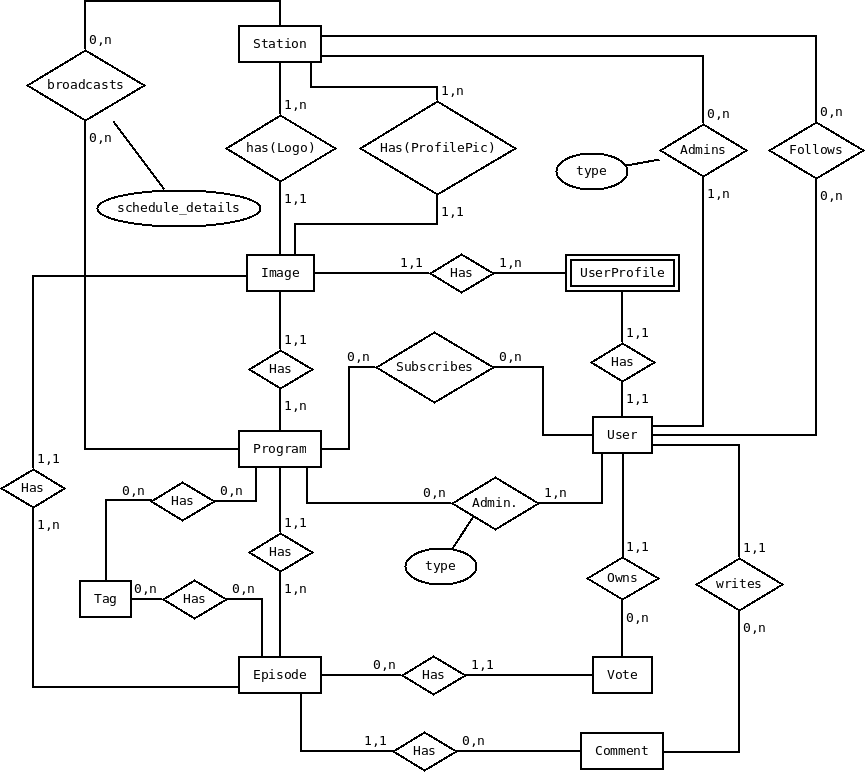
\includegraphics[scale=0.5,keepaspectratio=true]{./images/ER_diagrama.png}
	\caption{Diagrama Entidade-Relación da Base de Datos.}
	\label{fig:diagrama_er}
\end{figure}

\begin{figure}[h]
	\centering
	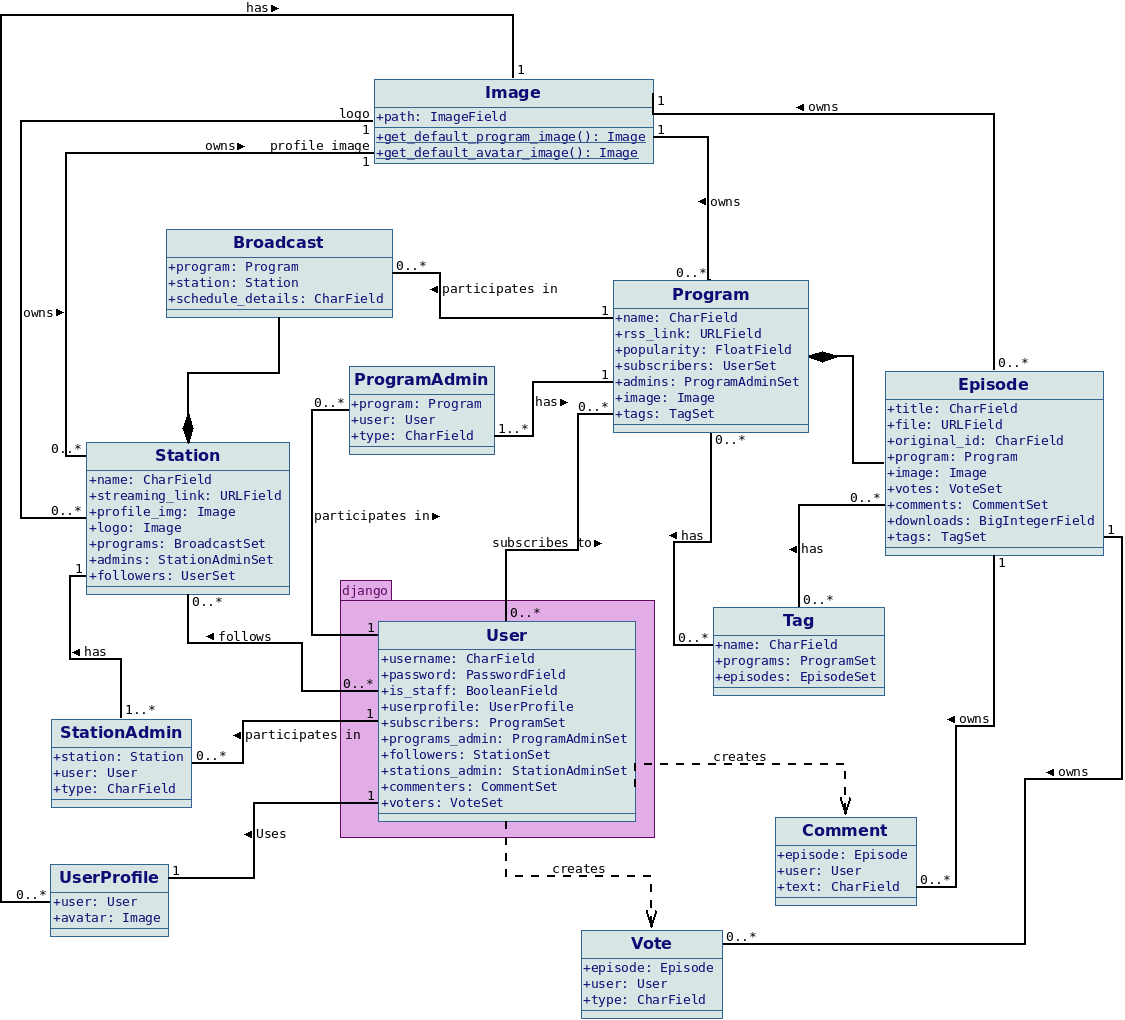
\includegraphics[scale=0.4,keepaspectratio=true]{./images/class_diagram.png}
	\caption{Diagrama de clases da capa modelo.}
	\label{fig:clase_models}
\end{figure}


\subsubsection{Usuarios}

Os usuarios están definidos por dúas táboas: \textbf{User} e \textbf{UserProfile} que se corresponden coas clases User, do paquete django.contrib.auth.models, e UserProfile, definida polo desenvolvedor e, polo tanto, incluída no módulo models.py. Esta segunda considerámola coma \textbf{feble} de User pois a existencia dun perfil está vencellada de xeito ineludible á existencia dun usuario (ver figura \ref{fig:diagrama_er}). Esta entidade auxiliar contén os atributos de usuario: avatar, descrición e localizción. Non se utiliza para máis nada.

A clase User inclúe os atributos necesarios para a \textbf{autenticación}: username, email e password, quedando este último encriptado en base de datos. De entre os campos utilizados para o funcionamento de Django, cómpre destacar is\_staff, que é o que concede acceso do usuario ao panel de administración da aplicación que provee o propio framework (como se mencionou no apartado \ref{django})

Outros atributos de User reflectidos na figura \ref{fig:clase_models} coma followers ou station\_admins son engadidos automáticamente polo framework ao declarar as relacións co fin de facilitar a navegación entre clases.


\subsubsection{Programas e episodios}

Entendemos, neste sistema, un programa coma un \textbf{produto radiofónico} do cal se publican entregas periodicamente. Están almacenados na táboa \textbf{Program} da base de datos. Os programas teñen, entre outros atributos, un nome, unha descrición, unha imaxe, un conxunto de categorías (táboa Tag) e un enlace a un \textbf{ficheiro RSS} dado polo usuario.

A \textbf{subscrición} dos usuarios aos programas modelouse coma unha relación N-N. As instancias de Program poden acceder ao conxunto dos seus subscritores mediante o atributo \textit{subscribers}.

\textbf{Episodio} é como chamamos ás entregas dun programa. Cada un ten, entre outros atributos, un enlace a un \textbf{ficheiro de audio} que será o que se poña a disposición dos usuarios na interface, un resumo, unha imaxe e un conxunto de etiquetas (tags). Un episodio ten que formar parte de 1 e só 1 programa. Se un programa é borrado, os episodios deixan de ter sentido no sistema e son borrados en cascada. Debido ao anterior, considérase a relación destas clases coma unha \textbf{composición}.


\subsubsection{Votos e comentarios}

Nunha primeira aproximación ao deseño da base de datos, entendéronse estas dúas entidades coma simples relacións N-N entre as entidades Episode e User. Porén, decidiuse finalmente que representan conceptos de seu que non perden o sentido semántico fóra da relación e, polo tanto, modeláronse coma entidades (Vote e Comment nos diagramas \ref{fig:diagrama_er} e \ref{fig:clase_models}).

O atributo \textbf{type} de Vote serve para lle dar significado ao voto: Positivo, negativo ou neutro.


\subsubsection{A entidade Station}

Identifícanse coa entidade \textbf{Station} os colectivos aos que se poidan asociar os programas: \textbf{Emisoras de radio} por ondas, emisoras de radio por internet ou canles de podcasting. O atributo mais destacable de Station é o de streaming\_link, que garda o enlace á canle de emisión por internet da emisora que será logo utilizado polo reproductor na web. Este campo pode ser nulo para aqueles colectivos que non dispoñan de emisión en directo.  

A emisión dos programas por parte das emisoras queda modelada coma unha relación N-N entre Program e Station á que chamamos \textbf{broadcasts}. Engadiuse o atributo adicional de schedule\_details, un campo de texto para os detalles de emsión: Horario, periodicidade... A clase correspondente en models.py é \textbf{Broadcast}. Dada a natureza de Station coma aglutinador de programas e dado que non ten sentido a existencia dunha emisión sen emisora, entendeuse que a relación entre Broadcast e Station é de \textbf{composición}. 


\subsubsection{Administración de contido}

Existe unha relación N-N entre os usuarios e as emisoras e unha semellante entre os usuarios e os programas: A de \textbf{administración}. Entendemos esta coma a posibilidade de editar, actualizar e borrar os contidos preexistentes. Isto queda reflectido nas clases \textbf{ProgramAdmin} e \textbf{StationAdmin}. As súas instancias relacionan, respectivamente, aos usuarios cos programas e emisoras que poden administrar e establecen os permisos de administración que posúen, estes últimos, expresados polo atributo type.

Tanto para a administración de emisoras como de Programas, existen dous \textbf{roles: Propietario e administrador}. O propietario ten permisos completos: Edición, actualización, borrado e xestión de administradores. O administrador só ten permisos de edición e actualización.  

Nótese que tal relación de administración non existe no caso dos episodios. Isto débese a que, ao ser engadidos automaticamente segundo a información recibida polo ficheiro RSS do programa (explicado máis en detalle na sección \ref{rss_parser_section}), non son editables. Aquelas opcións que poidan afectar en bloque aos episodios dun programa considéranse xa opcións do programa.

Os \textbf{superusuarios} do sistema, pola súa parte, poden editar e borrar calquera contido mediante ferramentas de Django coma o panel de administración ou o IPython shell.

\subsection{Deseño de interacción}

A figura \ref{fig:access_tree} mostra o mapa de navegación entre vistas. Isto serviu como guía do deseño das capas vista e template que se analizan a continuación.

\begin{figure}[h]
	\centering
	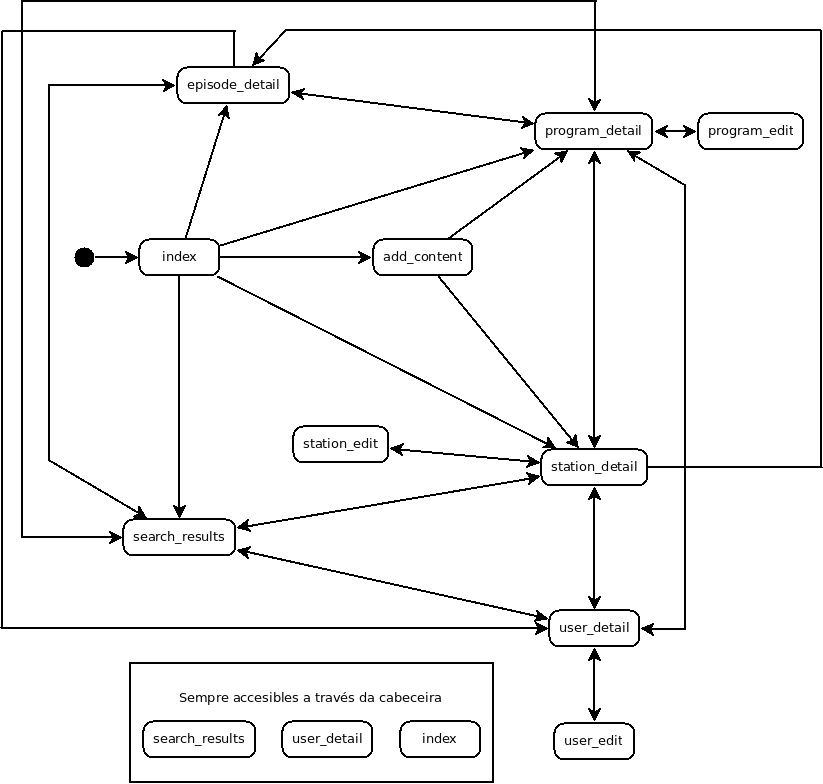
\includegraphics[scale=0.5,keepaspectratio=true]{./images/access_tree_auth.png}
	\caption{Mapa de navegación entre as distintas páxinas.}
	\label{fig:access_tree}
\end{figure}


\subsection{Capa Vista}

A capa vista é na que se atopa a \textbf{lóxica funcional da aplicación}. Fai uso dos obxectos da capa modelo para, ou ben extraer e compoñer os datos que serán enviados ao cliente, ou ben recoller os datos enviados desde o cliente para facer as conseguintes modificacións na base de datos. O módulo central desta capa é \textbf{views.py}. Nel, defínense funcións e clases que reciben un obxecto de Django \textbf{HttpRequest} e unha serie de parámetros opcionais e, tras realizar as operacións necesarias, retornan un obxecto \textbf{HttpResponse}.

Un obxecto HttpRequest contén metadatos da petición que se executou desde o cliente: Información da sesión do usuario, tipo de petición (GET, POST...), datos necesarios para os posibles \textbf{middlewares} e datos que o cliente envía a través dos formularios. 

Os middlewares, en Django, son plugins que alteran globalmente a entrada e saída do procesamento das peticións e as respostas. O framework oferta certa variedade de plugins de serie e a posibilidade de crear middlewares propios. Comentaranse os utilizados no capítulo de Implementación.

Un obxecto HttpResponse contén os datos que han de ser devoltos ao cliente, incluíndo a páxina á que se ha de redirixir ao usuario por causa da petición. Django require gardar os datos nun dicionario clave-valor ao que chama \textbf{context}. Esas claves valerán para acceder aos valores no template á hora de renderizar a resposta.

A decisión de a qué instancia ou función se lle pasa o obxecto HttpRequest tómase en base á url destino enviada polo cliente xunto co propio obxecto. É necesario manter un módulo que relacione as urls coas funcións e clases correspondentes á operación a realizar. Comunmente en Django e tamén neste proxecto, este ficheiro chámase \textbf{urls.py}.

Na figura \ref{fig:vista} amósase un esquema do funcionamento da capa vista. Para unha maior claridade, condensáronse as distintas clases de middleware nun único paso do diagrama. Tamén nesa figura pode verse unha referencia ao obxectos \textbf{Form} de Django que son utilizados neste proxecto. Estes obxectos consisten nunha abstracción de Python da información procedente dos formularios despregados no template e dos contedores de dita información (selectores, caixas de texto...). O seu uso é opcional, pero simplifican a definición valores por defecto e a \textbf{validación dos datos}.

\begin{figure}[H]
	\centering
	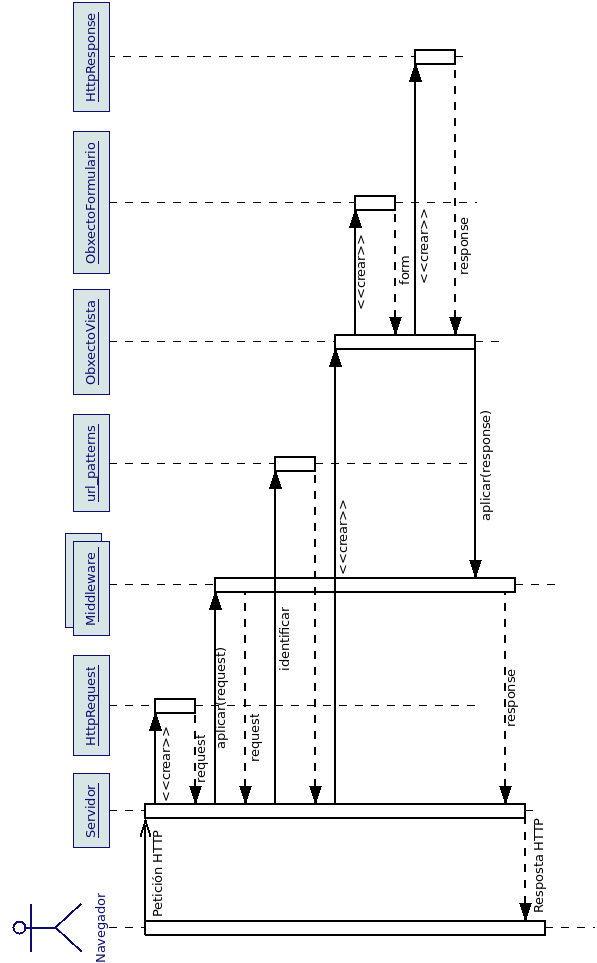
\includegraphics[scale=0.6,keepaspectratio=true]{./images/secuencia_vista_v.png}
	\caption{Esquema do funcionamento das vistas.}
	\label{fig:vista}
\end{figure} 

 


\subsubsection{Engadir contido}
\label{rss_parser_section}

Explicarase en detalle esta vista por ser, a posibilidade de que os usuarios engadan os seus propios programas e os episodios, a \textbf{parte principal deste proxecto}. Un usuario, pode engadir un programa e todos os seus episodios simplemente proporcionándolle á aplicación o enlace ao seu \textbf{ficheiro de RSS}.

\begin{figure}[h]
	\centering
	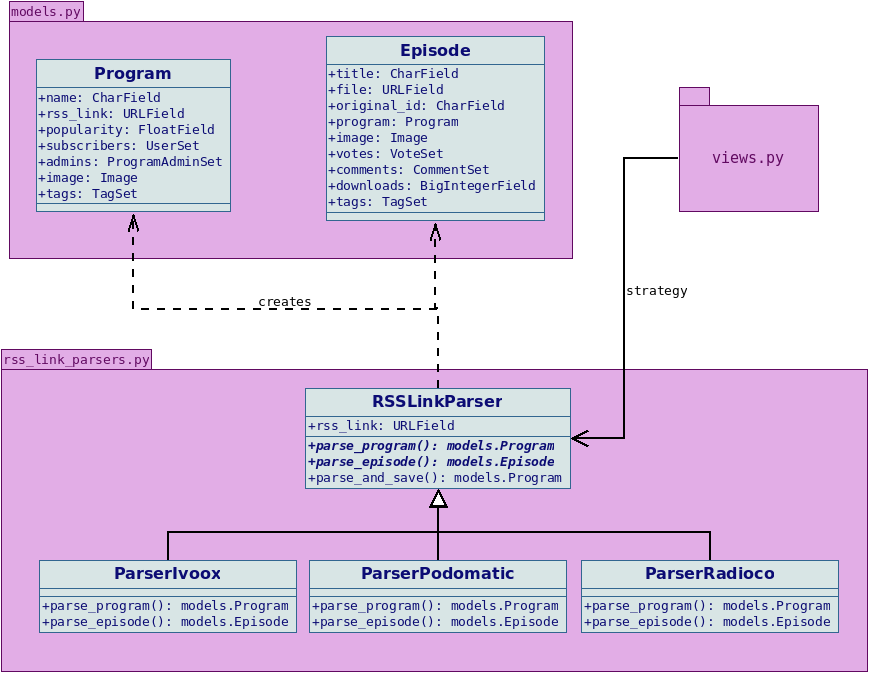
\includegraphics[scale=0.45,keepaspectratio=true]{./images/strategy.png}
	\caption{Patrón Estratexia utilizado para o procesamento de RSS.}
	\label{fig:strategy}
\end{figure}

A \textbf{función de vista} encargada de realizar este traballo recibe o obxecto de request e carga os datos deste nun formulario de Django. Unha vez validado, accede ao ficheiro RSS e extrae os datos do programa e os episodios. Enfrontámonos aquí a unha limitación do proxecto: Distintos servidores de podcasting poden ter \textbf{distintos formatos de ficheiro RSS}.

Debido a isto, debía deseñarse o sistema de xeito que puidésemos contar con distintos algoritmos de interpretación do RSS e, de cara a unha continuación do desenvolvemento, que engadir novos algoritmos fose sinxelo. De modo que se decidiu aplicar o \textbf{patrón de deseño \say{estratexia}}, como se ve no diagrama \ref{fig:strategy}. A superclase, \textbf{RSSLinkParser}, implementa o método \textit{parse\_and\_save}, encargado da creación das novas instancias. Esta función utiliza os métodos de lectura da información de programa e episodio, pero deixa a súa implementación ás clases fillas. Actualmente, o proxecto soporta \textbf{3 tipos ficheiro RSS} dos máis populares entre os usuarios obxectivo.


\subsection{Capa Template}
\label{capa_template}

A capa template define a \textbf{forma na que os datos} obtidos na capa vista \textbf{serán amosados} ao usuario e tamén os métodos de entrada de datos que poremos a disposición deste. A idea xeral foi a dunha interface na que os datos simples (atributos) se amosan en forma de lista e os complexos (Entidades) en \textbf{forma de cuadrícula}. Cada elemento desa cuadrícula representa un programa, episodio ou emisora da forma representada na figura \ref{fig:grella} e constitúe un enlace á páxina de detalles desa entidade.

\begin{figure}[H]
	\centering
	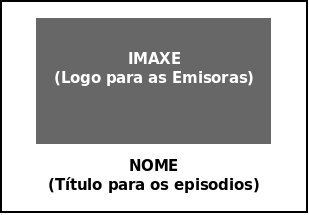
\includegraphics[scale=0.6,keepaspectratio=true]{./images/grella.png}
	\caption{Esquema dun elemento da cuadrícula.}
	\label{fig:grella}
\end{figure}

Pensando no uso da web en \textbf{dispositivos móbiles}, o número de elementos por fila da cuadrícula varía dependendo do tamaño da pantalla. Aquelas páxinas divididas de xeito horizontal (esquerda e dereita)  pasan a verticais (arriba e abaixo) pois considerase o \say{scroll} vertical máis cómodo para o usuario destes dispositivos. 

Todas as páxinas levan unha \textbf{cabeceira} amosando a información transversal á páxina: Un enlace á portada, botón de inicio/peche de sesión, unha caixa de procura por texto e máis o selector de linguaxe. 

A continuación coméntase brevemente as diferentes partes da interface:


\subsubsection{Portada}

Pensouse na portada coma unha páxina que ofreza \textbf{información breve e xeral} que o usuario queira consultar con máis frecuencia, por exemplo, as novidades nas súas subscricións e o acceso rápido ás súas emisoras favoritas. Tamén, pensando nos usuarios anónimos, considerouse engadir información de interese xeral coma os episodios máis recentes ou os programas máis \say{populares}, concepto que se explica na sección \ref{daemon_desenho}.

\begin{figure}[H]
	\centering
	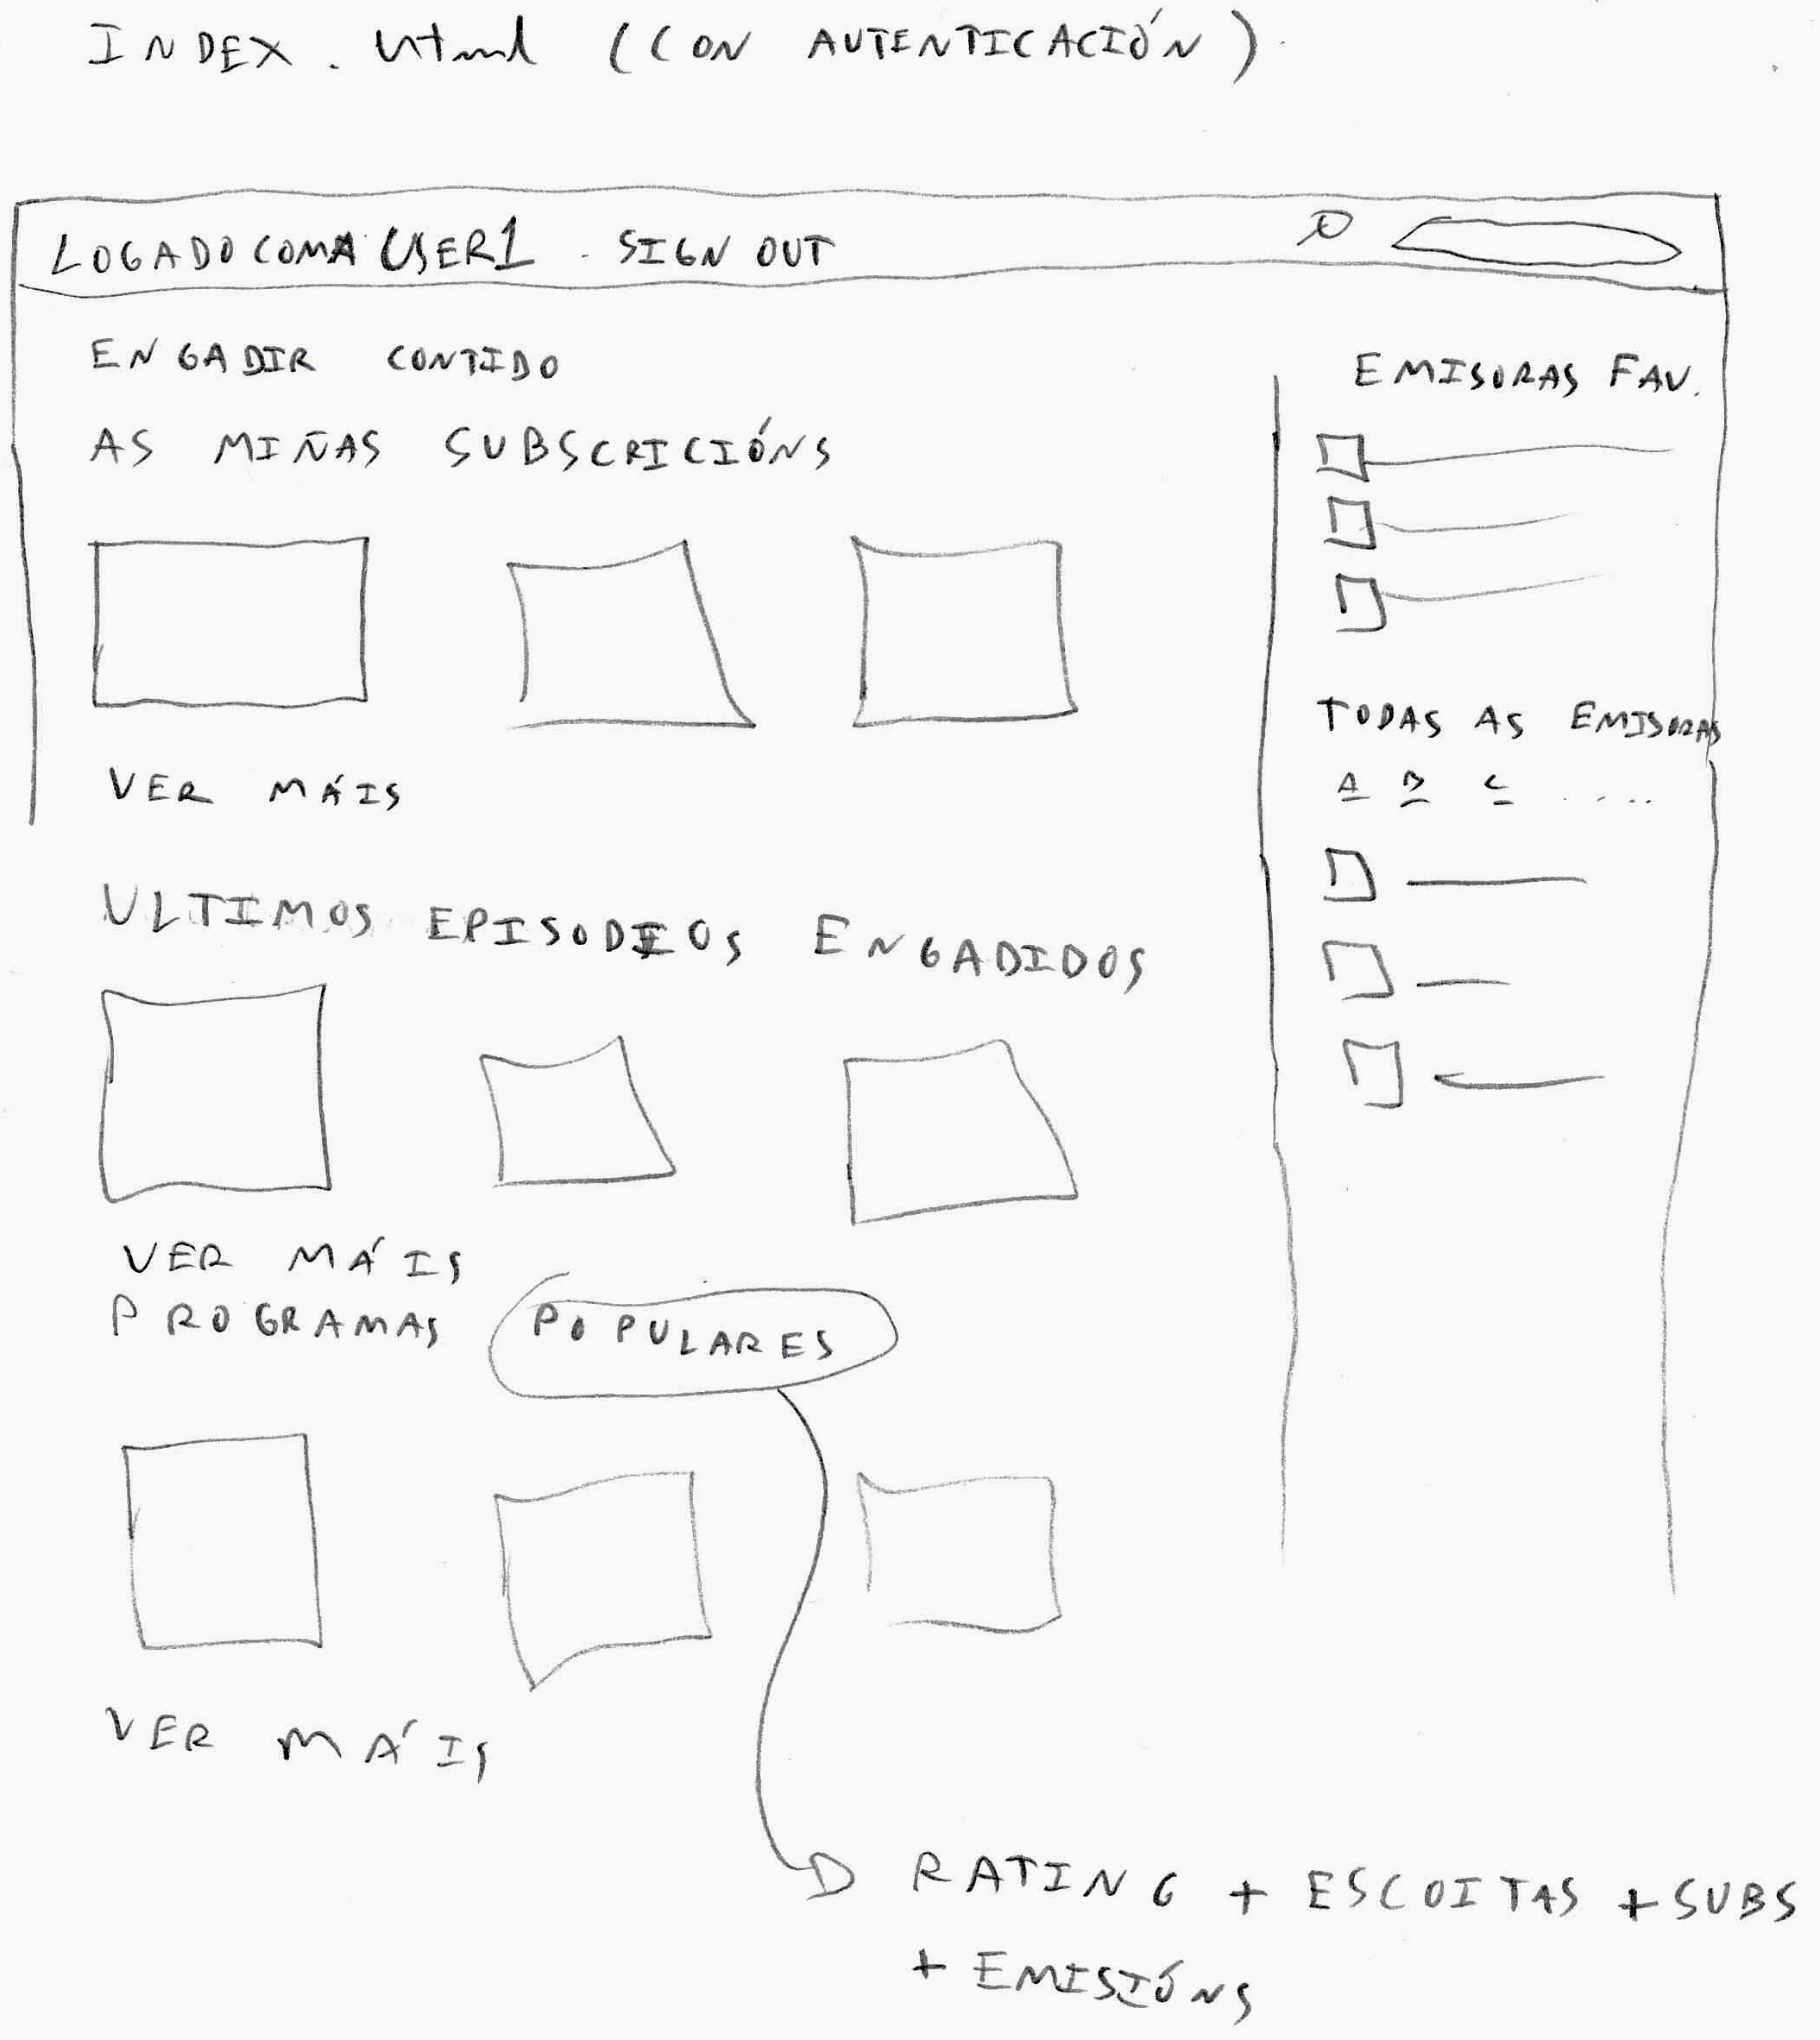
\includegraphics[scale=0.2,keepaspectratio=true]{./images/index1_p.png}
	\caption{Extracto do borrador do deseño da interface. Portada.}
	\label{fig:index1_p}
\end{figure}


\begin{figure}[h]
	\centering
	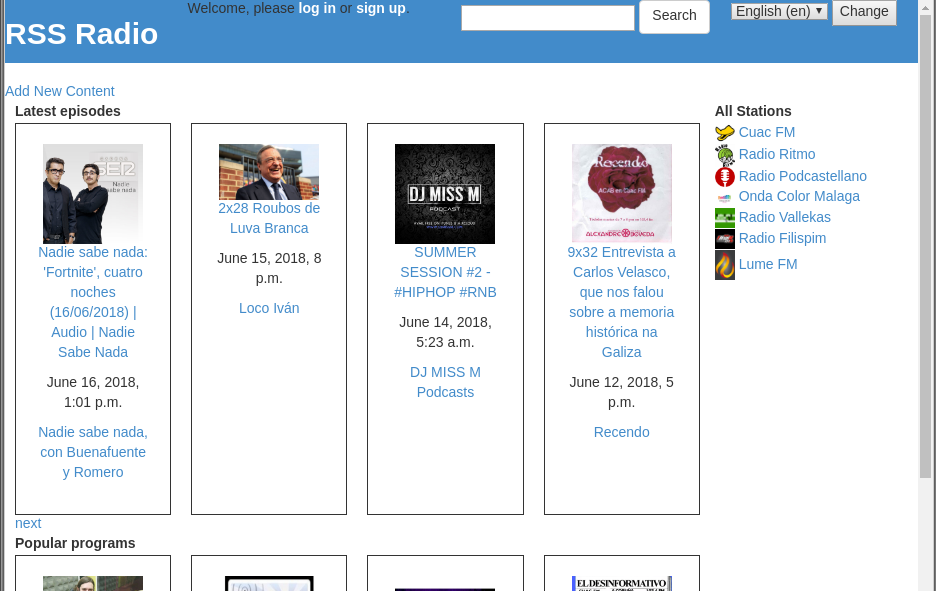
\includegraphics[scale=0.44,keepaspectratio=true]{./images/responsive1.png}
	\caption{Deseño final da portada.}
	\label{fig:responsive1}
\end{figure}

\begin{figure}[H]
	\centering
	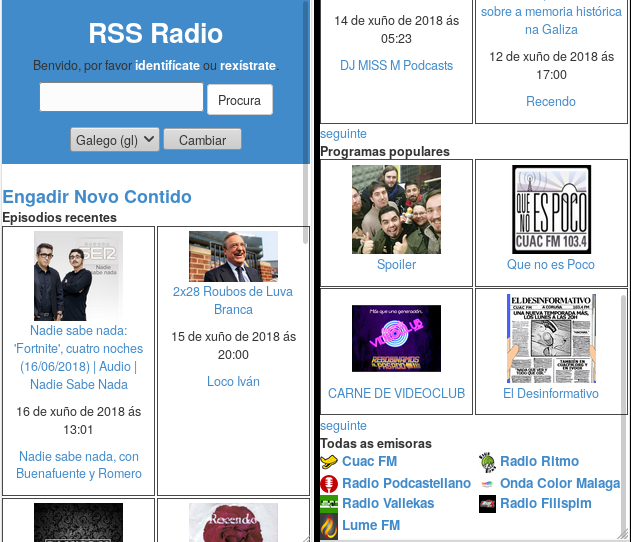
\includegraphics[scale=0.5,keepaspectratio=true]{./images/responsive2.png}
	\caption{Deseño da portada para dispositivos móbiles. Á esquerda, a parte superior, á dereita, a parte inferior.}
	\label{fig:responsive2}
\end{figure}


Na figura \ref{fig:index1_p} amósase un \textbf{primeiro borrador do deseño da interface} desta páxina. Móstrase a información dos programas e os episodios en forma de grella na parte esquerda e das emisoras en forma de lista no lado dereito. Isto cambia nos pequenos dispositivos, onde a información das emisoras pasa a situarse na parte máis baixa da páxina. Pódese ver este cambio comparando as figuras \ref{fig:responsive1} e \ref{fig:responsive2}.


\subsubsection{Páxinas de engadir e editar contido}

As páxinas de engadir contido (incluída a de rexistrar usuario) consisten na lista de atributos da entidade a engadir xunto cos seus respectivos elemento HTML de entrada de datos. As de edición son semellantes, pero amosando os valores actuais da entidade.

\subsubsection{Páxinas de detalle}

Ás páxinas de detalle son aquelas onde se amosa a \textbf{información completa dunha instancia} dalgunha das 4 grandes clases deste proxecto: Usuario, emisora, programa e episodio. Tamén debería dar acceso á páxina de edición de ter, o usuario, permisos para iso.

Na figura \ref{fig:program1_p} amosamos un borrador do deseño da interface da páxina de detalles de programa que nos ha valer coma exemplo xeral: Encabézase coa imaxe da instancia e o seu nome. Debaixo, lístanse os seus atributos incluíndo o reprodutor de audio para os casos de emisora e episodio. Finalmente, as \textbf{cuadrículas} dos obxectos cos que se relacionan.

A máis distinta sería, se cadra, a de episodio. Esta incluiría ao final unha \textbf{sección de comentarios} en lugar dunha grella de obxectos.


\subsubsection{Páxina de resultados de busca}

A páxina de resultados de busca é á que se accede a través da \textbf{caixa de procura da cabeceira} (busca por texto) ou a través de \say{clicar} nunha etiqueta de categoría (busca por tag). Divídese en dúas partes en proporcións semellantes á de portada: A parte da esquerda amosa as entidades atopadas en forma de cuadrícula e a da dereita unha \textbf{nube de etiquetas}.

\begin{figure}[H]
	\centering
	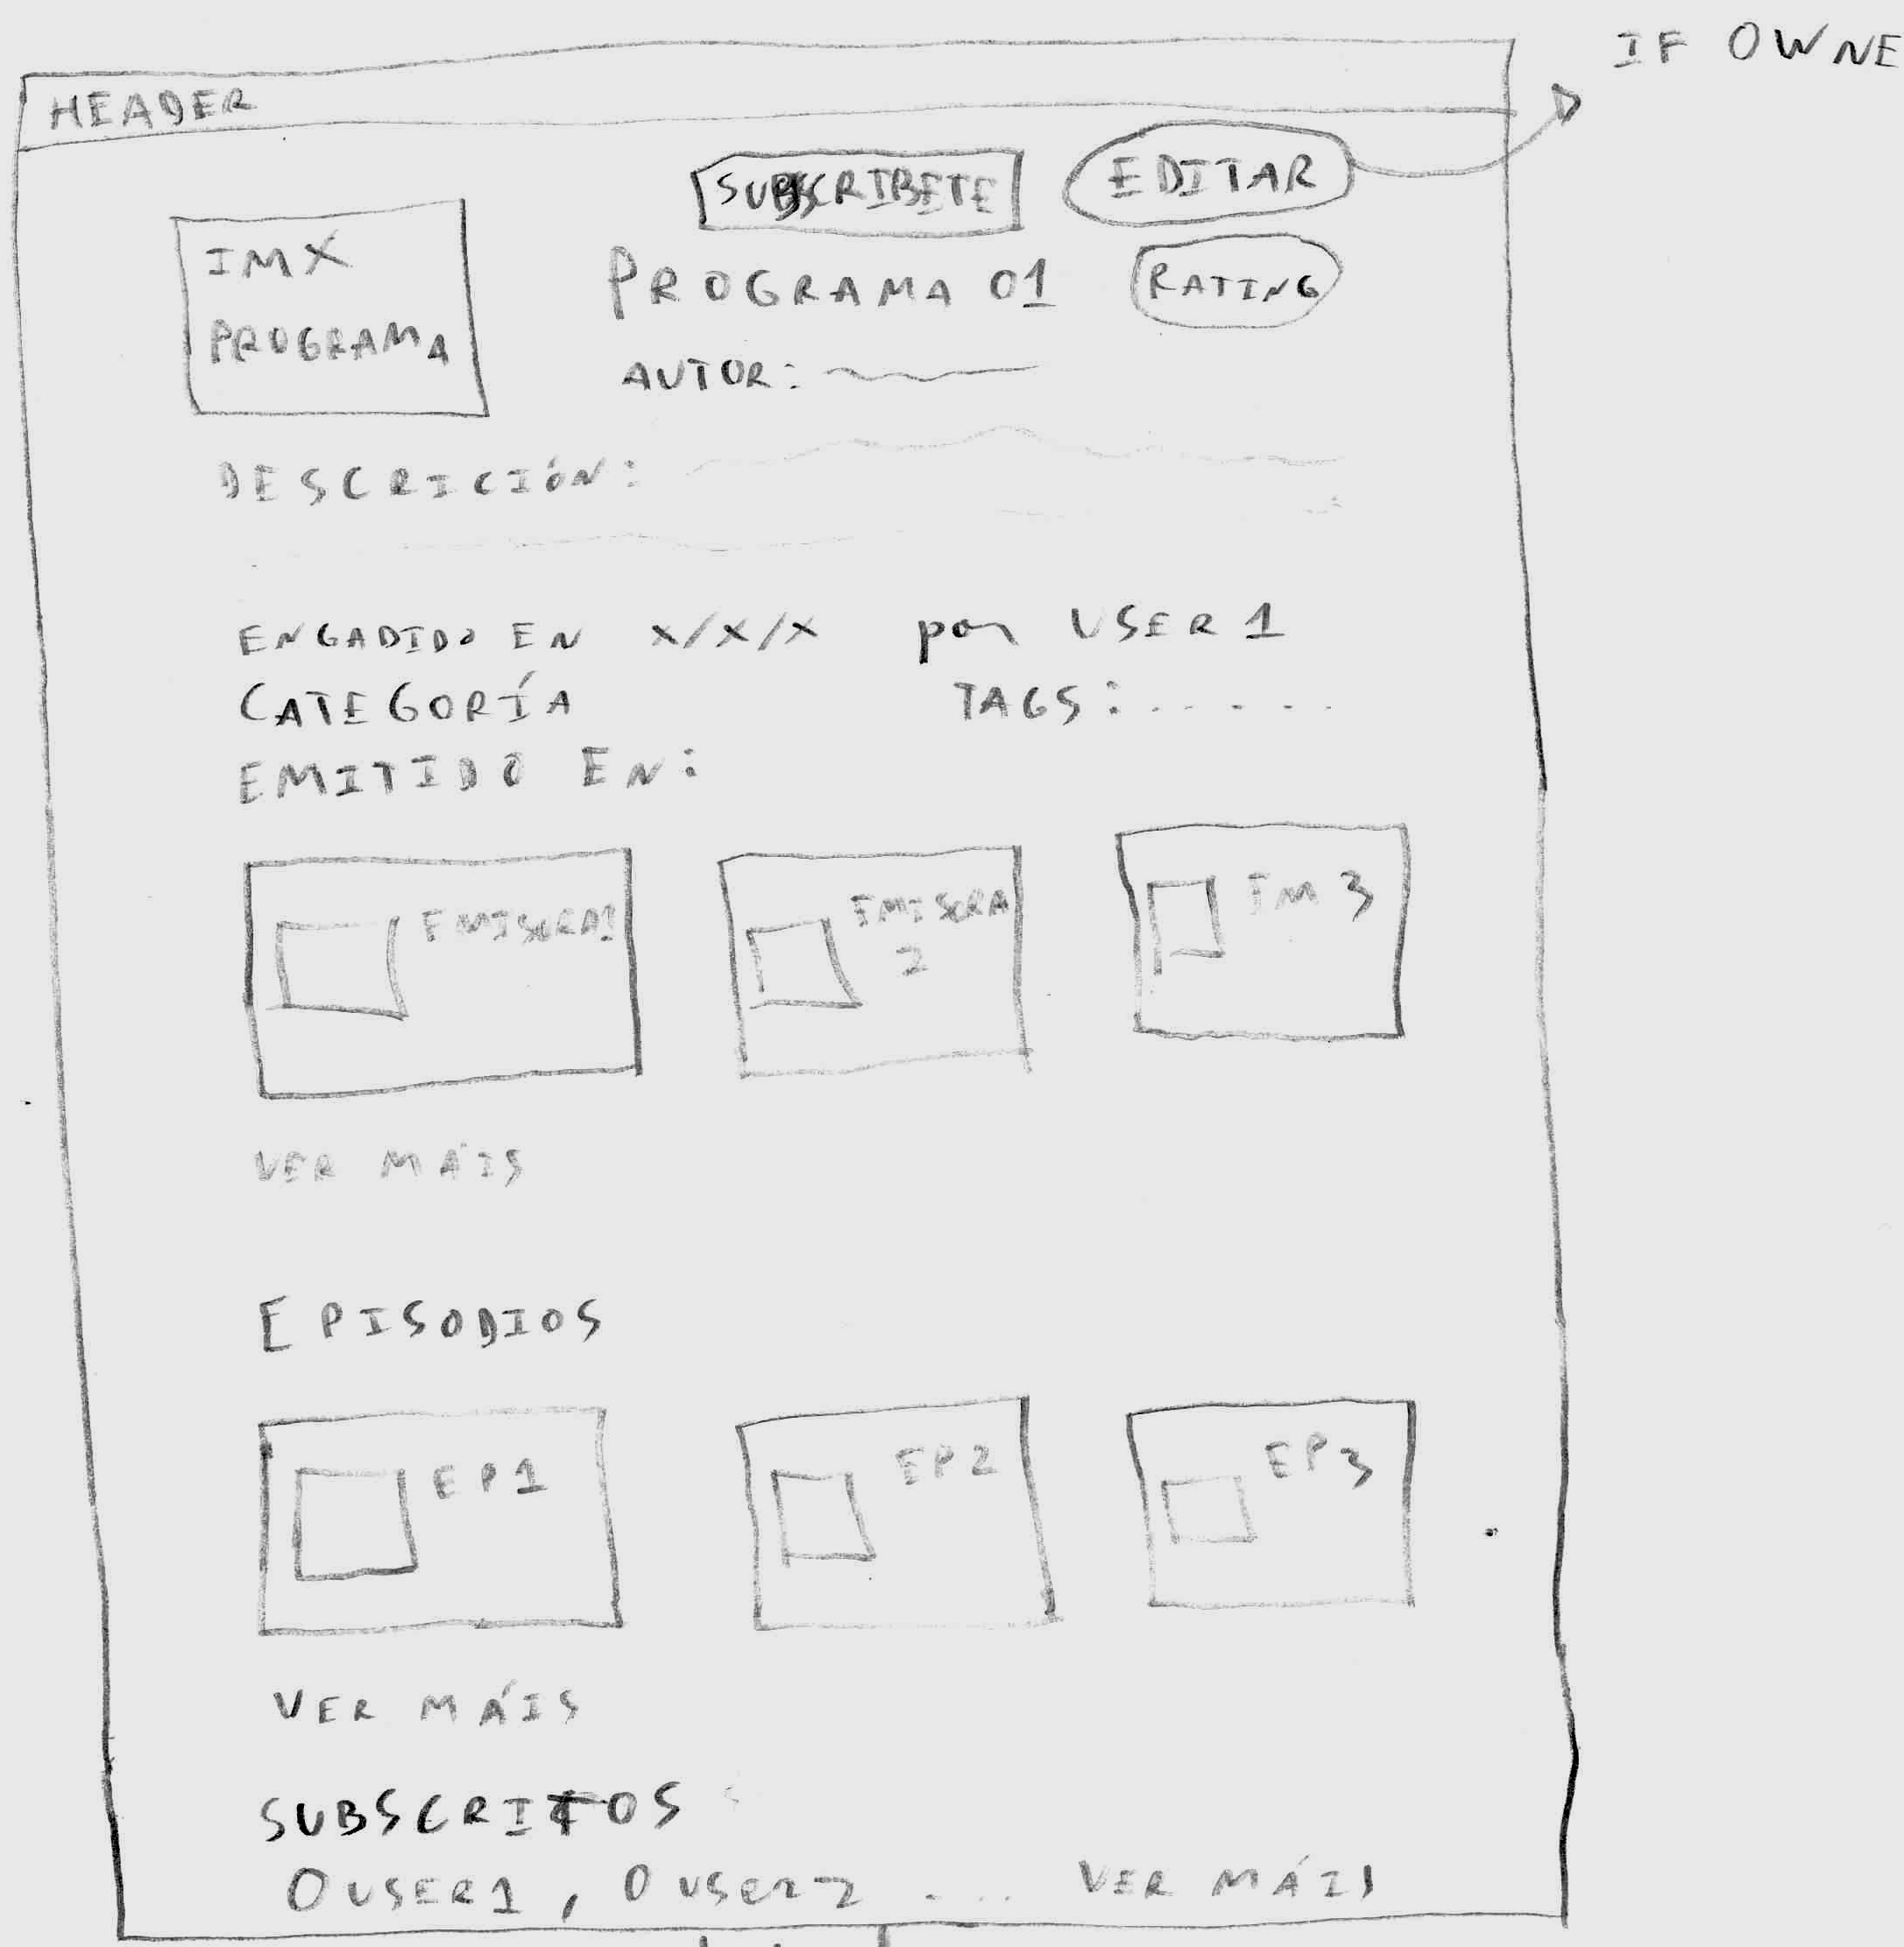
\includegraphics[scale=0.2,keepaspectratio=true]{./images/program1_p.png}
	\caption{Extracto do borrador do deseño da interface. Detalles de programa.}
	\label{fig:program1_p}
\end{figure}


\subsubsection{Páxinas de xestión}

As páxinas de xestión de emisión e xestión de administradores para programas e emisoras son semellantes. A figura \ref{fig:manage1_p} mostra un esquema de interface da páxina que permitiría xestionar os \textbf{programas emitidos por unha emisora}. Aínda que o aspecto aí debuxado cambiou moito durante a implementación, serve para dar unha idea das necesidades de deseño: O usuario xestor ten que poder ver os programas xa emitidos para poder eliminalos da emisión e ver os non emitidos para poder engadilos ao catálogo da emisora.


\begin{figure}[H]
	\centering
	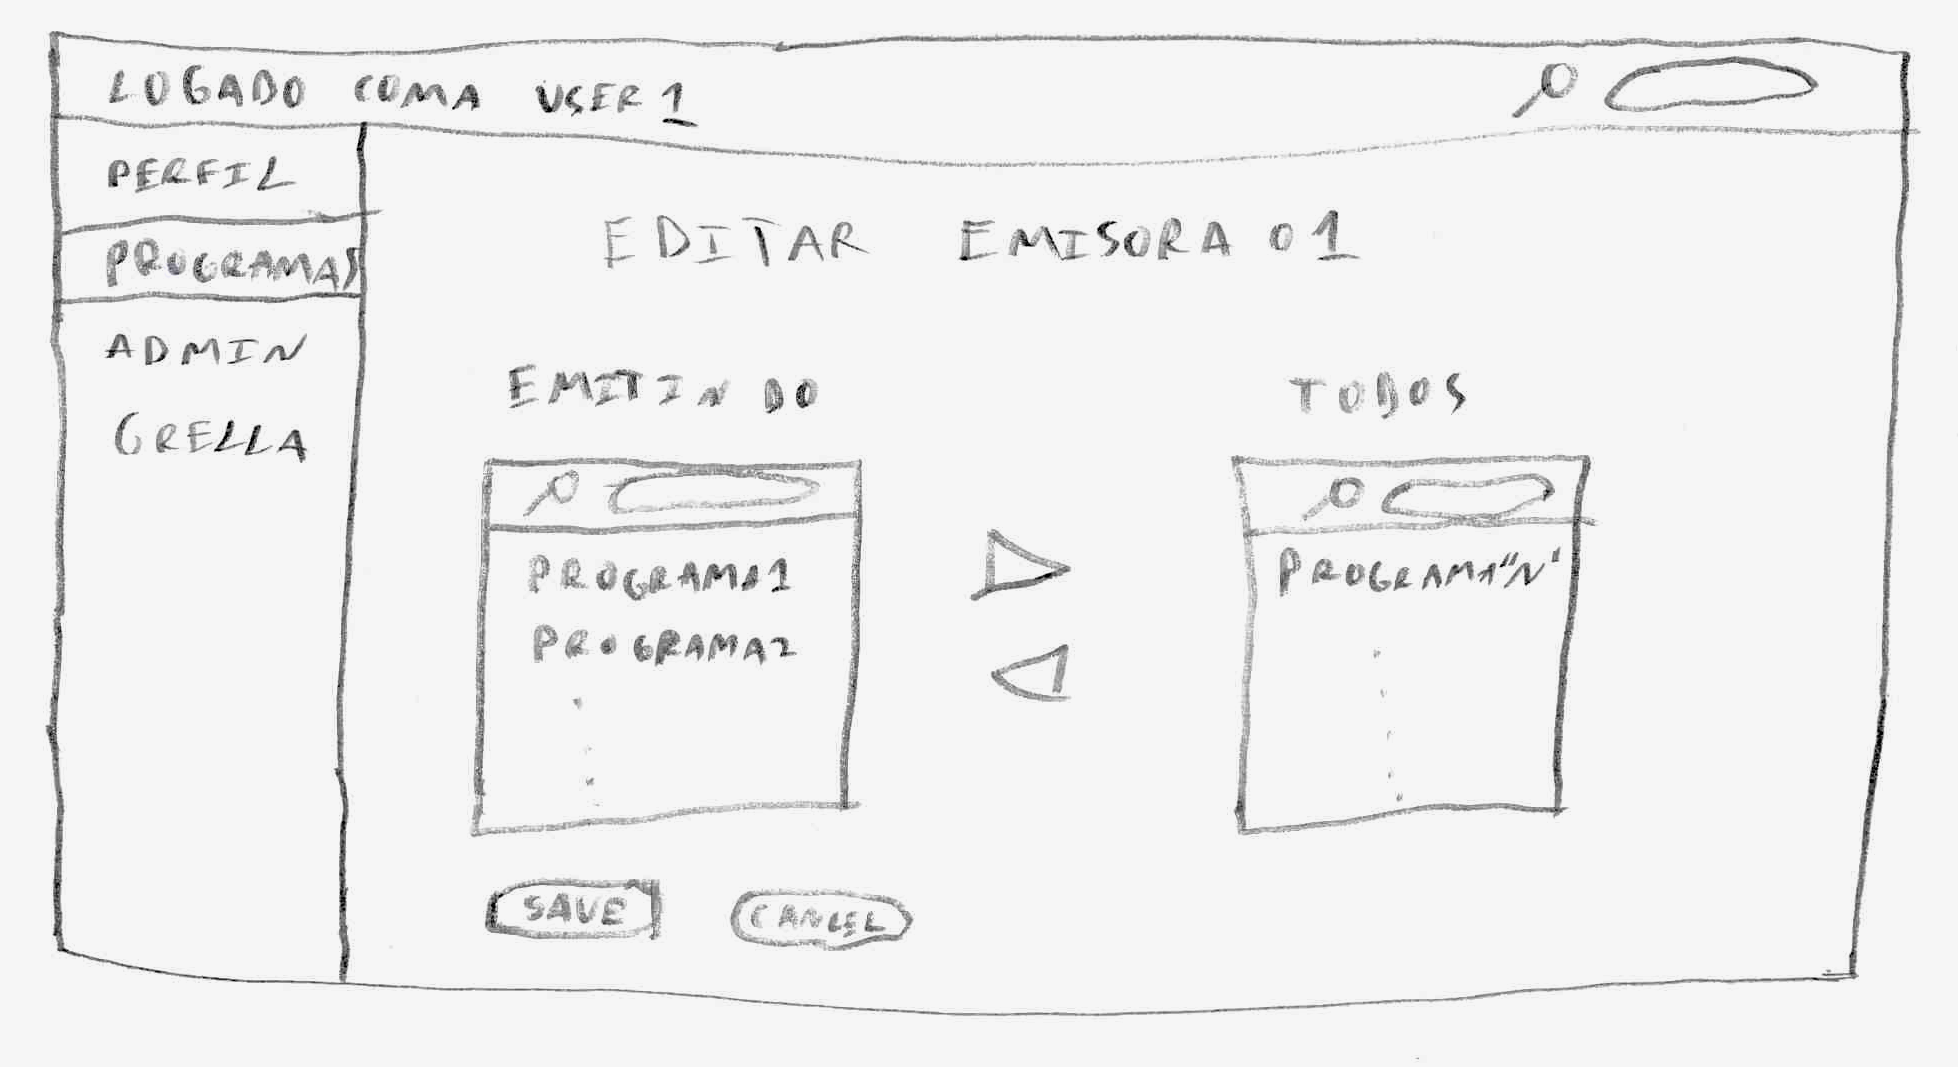
\includegraphics[scale=0.2,keepaspectratio=true]{./images/manage1_p.png}
	\caption{Extracto do borrador do deseño da interface. Xestión de emisión.}
	\label{fig:manage1_p}
\end{figure}



\section{Actualización dos datos}
\label{daemon_desenho}

Existen dous \textbf{procesos executados periodicamente} no lado do servidor co fin de manter actualizados os datos dos programas no sistema.

\subsubsection{Novos episodios}

Cando un programa é engadido, todos os episodios presentes no ficheiro RSS gárdanse tamén. A partir de entón, é responsabilidade do sistema facer \textbf{polling do RSS} para detectar as novas publicacións e engadilas á base de datos. Este proceso reutiliza o código do módulo rss\_link\_parsers visto na sección \ref{rss_parser_section}.

\subsubsection{Popularidade e cualificación dos programas}

A \textbf{cualificación} (rating) dun programa calcúlase en base aos \textbf{votos positivos e negativos}. Só se teñen en conta os episodios con data de publicación entre os últimos 365 días. Se non hai votos, asúmese unha cualificación do 50\%:

\[cualificacion_{p}=100\frac{\sum_{episodios_p}vpositivos}{\sum_{episodios_p}vpositivos+vnegativos}\]

A \textbf{popularidade} é unha medida do impacto que os programas teñen no sistema e, coma tal, inflúe na súa \textbf{visibilidade} en portada e resultados de procura. Depende das subscricións, dos votos ponderados dos episodios, das escoitas dos episodios e do número de emisoras que o emitan. Tampouco aquí se teñen en conta os episodios con máis dun ano de antigüidade.

\[vponderados_e=(vpositivos-vnegativos)*(vpositivos+vnegativos)\]
\[popularidade_{p}=5*subscricions+10*emisoras+escoitas+\sum_{episodios_p}vponderados_e\]

A ponderación de emisoras e subscricións decidiuse en base a \textbf{diferencia de magnitude} esperada. A ponderación dos votos é en base ao número de votos de cada capítulo.

Ámbolos dous valores, ao depender de actividades dos usuarios, han de ser actualizados periodicamente.


